\section{Pretrained Lightweight Models}
\textbf{Owner: Lavanathan.J -- 230371R}

Two lightweight ImageNet-initialized architectures were evaluated using transfer learning. In both cases, the pretrained backbone was frozen and only a new classification head was trained. The head consisted of global average pooling, dropout with rate 0.2, and a five-unit Softmax classifier. No backbone fine-tuning or unfreezing was performed.

\subsection{MobileNetV2}

MobileNetV2 is designed for efficient visual recognition using inverted residual blocks and linear bottlenecks \cite{mobilenetv2}. The model was trained with $224\times224\times3$ inputs and MobileNetV2 preprocessing.

\begin{figure}[H]
\centering
\begin{subfigure}{0.48\linewidth}
\centering
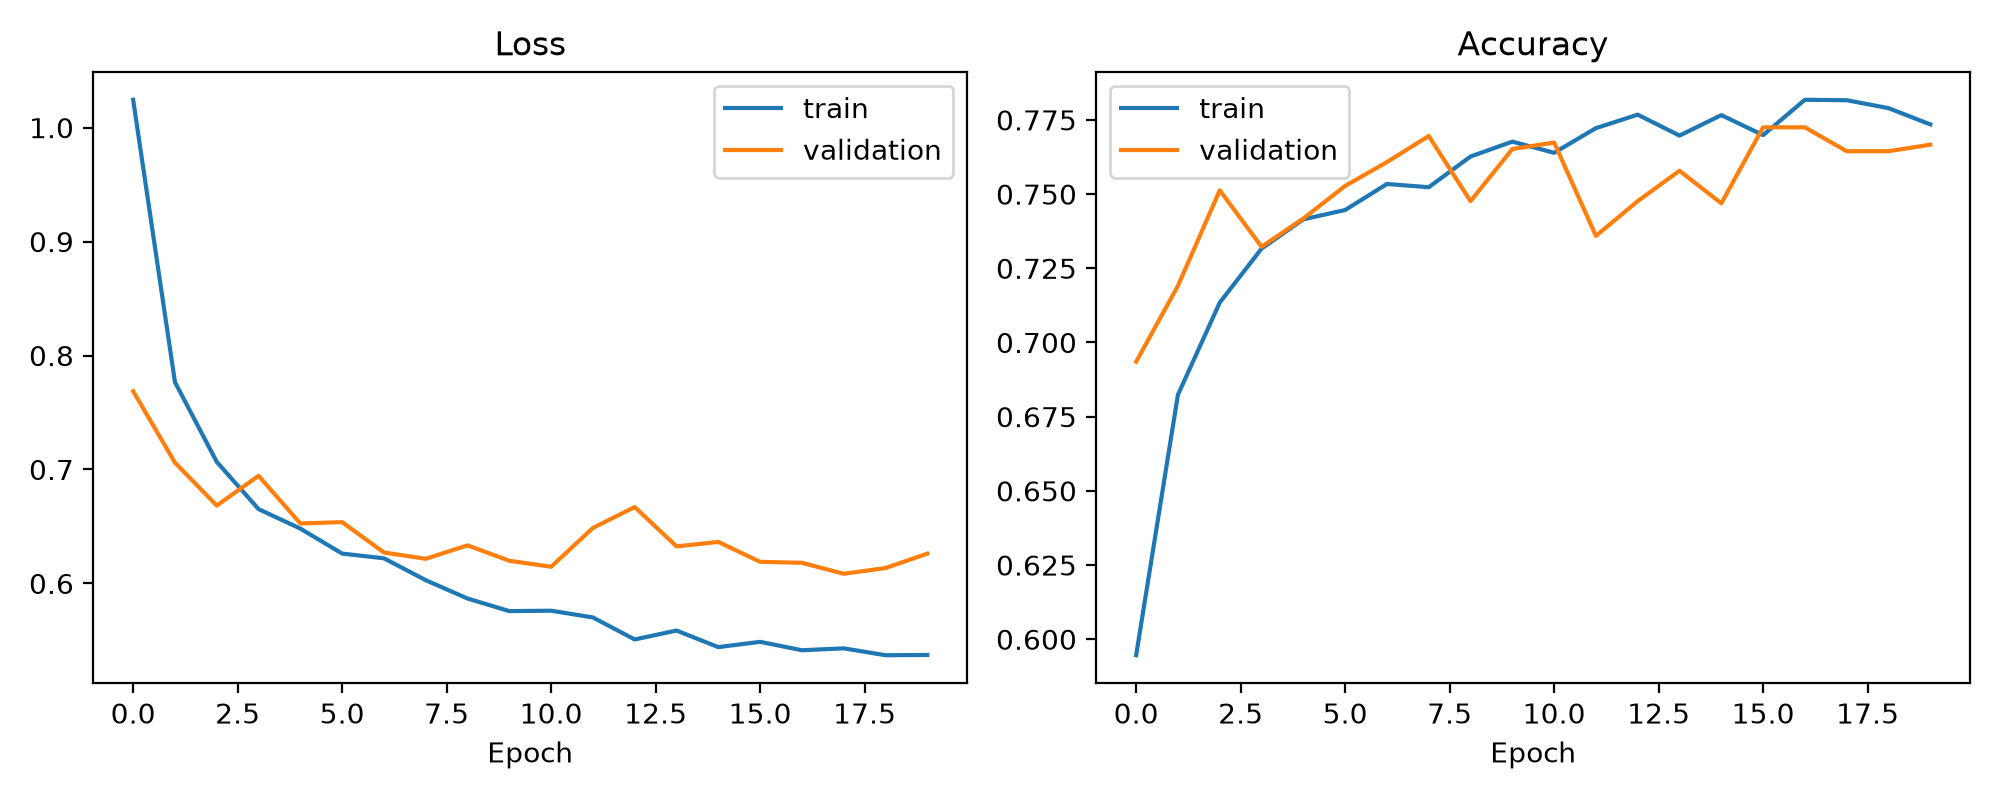
\includegraphics[width=\linewidth]{figures/mobilenetv2_history.png}
\caption{MobileNetV2 learning curves.}
\label{fig:mobilenet_history}
\end{subfigure}
\hfill
\begin{subfigure}{0.48\linewidth}
\centering
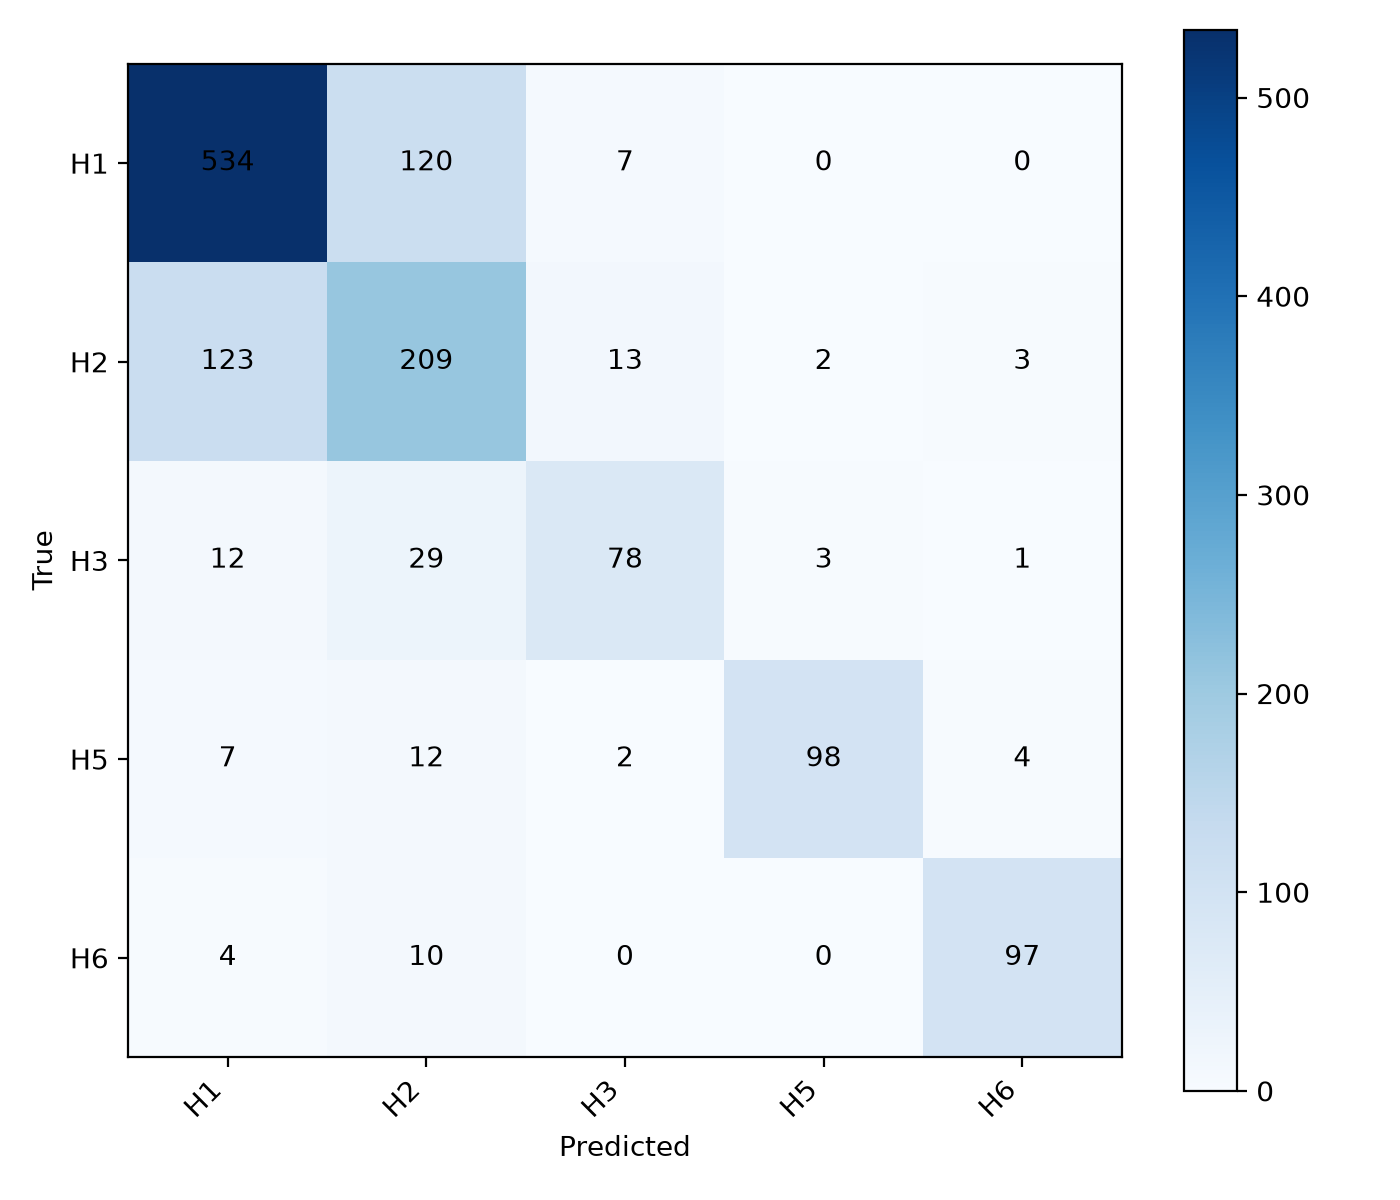
\includegraphics[width=\linewidth]{figures/mobilenetv2_confusion_matrix.png}
\caption{MobileNetV2 confusion matrix.}
\label{fig:mobilenet_confusion}
\end{subfigure}
\caption{MobileNetV2 transfer-learning evaluation.}
\end{figure}

\begin{table}[H]
\centering
\caption{MobileNetV2 results.}
\label{tab:mobilenet_results}
\begin{tabular}{lr}
\toprule
Metric & Value \\
\midrule
Total parameters & 2,264,389 \\
Trainable parameters & 6,405 \\
Saved model size & 9.25 MB \\
Mean epoch time & 100.5135 s \\
Test accuracy & 0.7427 \\
Macro precision & 0.7981 \\
Macro recall & 0.7420 \\
Macro F1-score & 0.7668 \\
\bottomrule
\end{tabular}
\end{table}

\subsection{EfficientNetB0}

EfficientNet uses compound scaling to balance network width, depth, and input resolution \cite{efficientnet}. EfficientNetB0 was trained with $224\times224\times3$ inputs and EfficientNet preprocessing.

\begin{figure}[H]
\centering
\begin{subfigure}{0.48\linewidth}
\centering
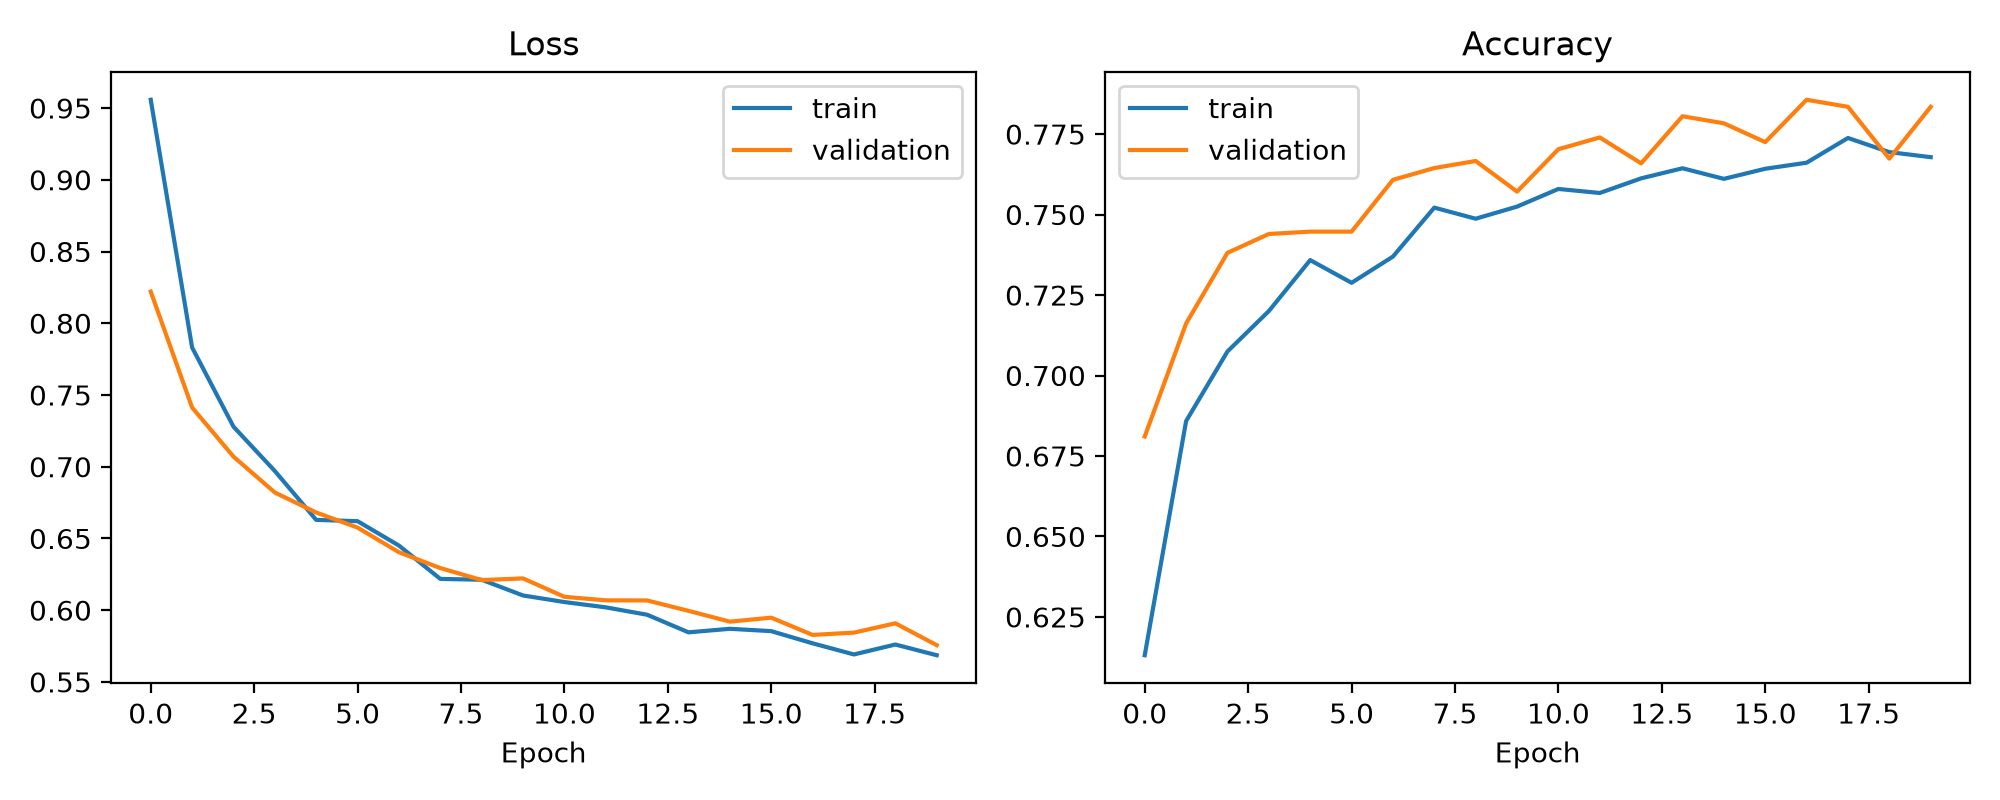
\includegraphics[width=\linewidth]{figures/efficientnetb0_history.png}
\caption{EfficientNetB0 learning curves.}
\label{fig:efficientnet_history}
\end{subfigure}
\hfill
\begin{subfigure}{0.48\linewidth}
\centering
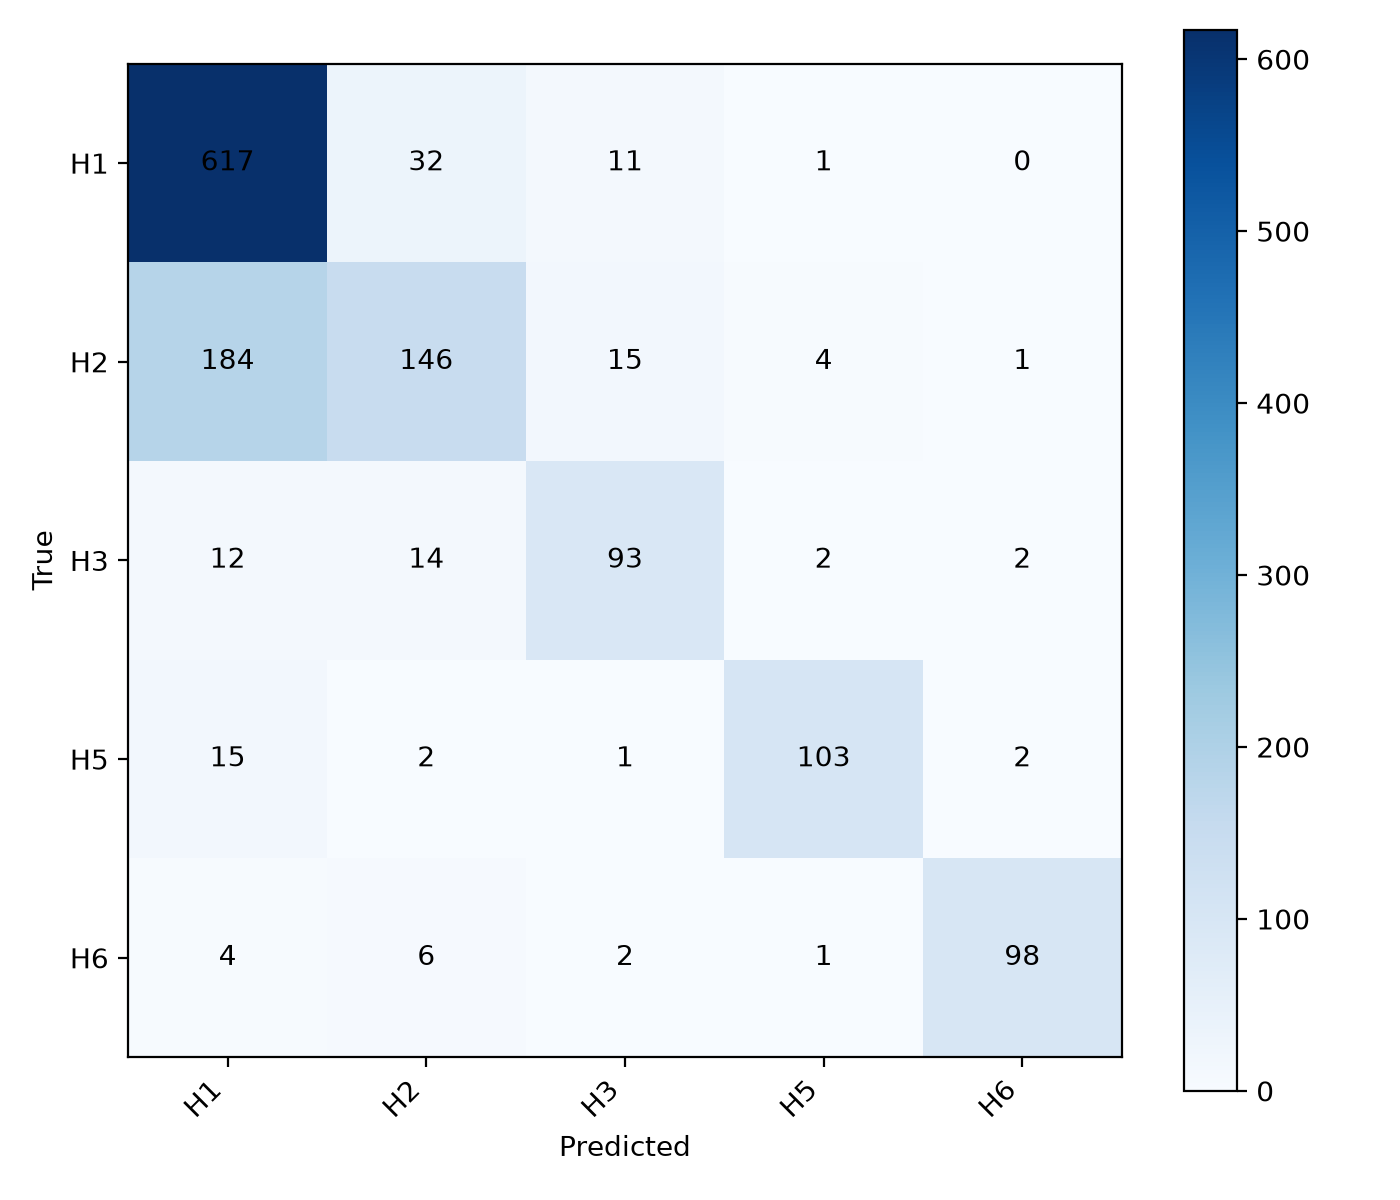
\includegraphics[width=\linewidth]{figures/efficientnetb0_confusion_matrix.png}
\caption{EfficientNetB0 confusion matrix.}
\label{fig:efficientnet_confusion}
\end{subfigure}
\caption{EfficientNetB0 transfer-learning evaluation.}
\end{figure}

\begin{table}[H]
\centering
\caption{EfficientNetB0 results.}
\label{tab:efficientnet_results}
\begin{tabular}{lr}
\toprule
Metric & Value \\
\midrule
Total parameters & 4,055,976 \\
Trainable parameters & 6,405 \\
Saved model size & 16.33 MB \\
Mean epoch time & 158.3490 s \\
Test accuracy & 0.7727 \\
Macro precision & 0.8227 \\
Macro recall & 0.7654 \\
Macro F1-score & 0.7826 \\
\bottomrule
\end{tabular}
\end{table}
